\documentclass[]{standalone}

\usepackage{amsmath}
\usepackage{amsfonts}
\usepackage{amssymb}
\usepackage{graphicx}
\usepackage{tikz}
\usepackage{import}
\usepackage[subpreambles=true]{standalone}

\usepackage{tikz}
\usepackage{tikz-3dplot}

\usetikzlibrary{positioning}
\begin{document}

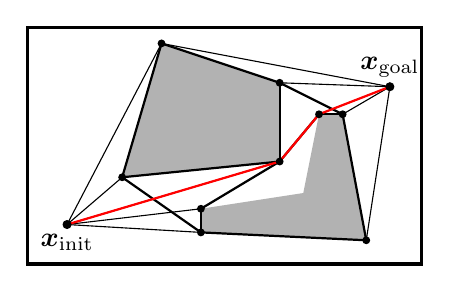
\begin{tikzpicture}[scale=1]
    \useasboundingbox (0,0) rectangle (5,3);
    
    \path[draw, very thick] (0,0) -- (5,0) -- (5,3) -- (0,3) -- cycle;
    
    \coordinate (obs1) at (2.4,2.1);
    \coordinate (obs2) at (3.7,0.65);
    
    \path[fill=black!30] (obs1) ++(-1.2,-1) -- ++(2,0.2) -- ++(0,1) -- ++(-1.5,0.5) -- cycle;
    \path[fill=black!30] (obs2) ++(-1.5,-0.25) -- ++(0,0.3) -- ++(1.3,0.2) -- ++(0.2,1) -- ++(0.3,0) -- ++(0.3,-1.6) -- cycle;
    
    \coordinate (init) at (0.5,0.5);
    \coordinate (goal) at (4.6,2.25);
    
    
    
    % consecutive reflex vertices obs 1
    \path[draw, thick] (1.2,1.1) -- (3.2,1.3);
    \path[draw, thick] (3.2,1.3) -- (3.2,2.3);
    \path[draw, thick] (3.2,2.3) -- (1.7,2.8);
    \path[draw, thick] (1.7,2.8) -- (1.2,1.1);
    
    % consecutive reflex vertices obs 2
    \path[draw, thick] (2.2,0.4) -- (2.2,0.7);
    \path[draw, thick] (2.2,0.4) -- (4.3,0.3);
    \path[draw, thick] (4.3,0.3) -- (4.0,1.9);
    \path[draw, thick] (3.7,1.9) -- (4.0,1.9);
    
    % bitangent edges
    \path[draw, thick] (1.2,1.1) -- (2.2,0.4);
    \path[draw, thick] (3.2,2.3) -- (4.0,1.9);
    \path[draw, thick] (3.2,1.3) -- (3.7,1.9);
    \path[draw, thick] (3.2,1.3) -- (2.2,0.7);
    
    % start and goal to all visible vertices
    % start
    \path[draw] (init) -- (1.2,1.1);
    \path[draw] (init) -- (2.2,0.4);
    \path[draw] (init) -- (2.2,0.7);
    \path[draw] (init) -- (1.7,2.8);
    \path[draw] (init) -- (3.2,1.3);
    
    % goal
    \path[draw] (goal) -- (1.7,2.8);
    \path[draw] (goal) -- (3.2,2.3);
    \path[draw] (goal) -- (4.3,0.3);
    \path[draw] (goal) -- (4.0,1.9);
    \path[draw] (goal) -- (3.7,1.9);
    
    % goal path
    \path[draw=red, thick] (init) -- (3.2,1.3) -- (3.7,1.9) -- (goal);

    
    % reflex vertices obs 1
    \path[fill=black] (1.2,1.1) circle (0.05);
    \path[fill=black] (3.2,1.3) circle (0.05);
    \path[fill=black] (3.2,2.3) circle (0.05);
    \path[fill=black] (1.7,2.8) circle (0.05);
    
    % reflex vertices obs 2
    \path[fill=black] (2.2,0.4) circle (0.05);
    \path[fill=black] (2.2,0.7) circle (0.05);
    \path[fill=black] (3.7,1.9) circle (0.05);
    \path[fill=black] (4.0,1.9) circle (0.05);
    \path[fill=black] (4.3,0.3) circle (0.05);

    % init and goal
    \path[draw, fill] (init) circle (0.05) node[below] {$\boldsymbol{x}_\mathrm{init}$};
    \path[draw, fill] (goal) circle (0.05) node[above] {$\boldsymbol{x}_\mathrm{goal}$};
\end{tikzpicture}
\end{document}